\documentclass{beamer}
%
% Choose how your presentation looks.
%
% For more themes, color themes and font themes, see:
% http://deic.uab.es/~iblanes/beamer_gallery/index_by_theme.html
%
\mode<presentation>
{
  \usetheme{default}      % or try Darmstadt, Madrid, Warsaw, ...
  \usecolortheme{default} % or try albatross, beaver, crane, ...
  \usefonttheme{default}  % or try serif, structurebold, ...
  \setbeamertemplate{navigation symbols}{}
  \setbeamertemplate{caption}[numbered]
} 

\usepackage[english]{babel}
\usepackage[utf8]{inputenc}
\usepackage[T1]{fontenc}
\usepackage{graphicx} % Required for inserting images
\usepackage{amsmath}
\usepackage{amsfonts}
\usepackage{amssymb}
\usepackage{amsthm}
\usepackage{tikz}
\usetikzlibrary{tikzmark}
\usepackage{braket}

\title[Your Short Title]{Measurement Based Quantum Computation}
\author{Yiting Pei}
\date{\today}

\begin{document}
\begin{frame}
  \titlepage
\end{frame}

\section{Preliminary: Quantum Teleportation}
\begin{frame}{Quantum Teleportation}
Input state: $\ket{\psi} = \alpha \ket{0} + \beta \ket{1}$. Initially, we have a 3-qubit state on $\textcolor{red}{\mathbb{C}^2}\otimes\textcolor{red}{\mathbb{C}^2}\otimes\textcolor{blue}{\mathbb{C}^2}$
\begin{align*}
    \ket{\Psi} = \textcolor{red}{\ket{\psi}} \otimes \frac{1}{\sqrt{2}} \left(\textcolor{red}{\ket{0}} \otimes \textcolor{blue}{\ket{0}} + \textcolor{red}{\ket{1}} \otimes \textcolor{blue}{\ket{1}}\right)
\end{align*}
\textcolor{red}{Alice} / \textcolor{blue}{Bob}
\end{frame}

\begin{frame}{Quantum Teleportation II}
    \begin{itemize}
        \item Alice performs a unitary transformation $U = (H \otimes \mathbb{I})CNOT$. The state becomes
        \begin{align*}
            \ket{\Psi'} = \textcolor{red}{\ket{00}}\textcolor{blue}{\ket{\psi}} + \textcolor{red}{\ket{01}}(\textcolor{blue}{\alpha\ket{1} + \beta\ket{0}}) + \textcolor{red}{\ket{10}}(\textcolor{blue}{\alpha\ket{0} - \beta\ket{1}}) \\+ \textcolor{red}{\ket{11}}(\textcolor{blue}{\alpha\ket{1} - \beta\ket{0}})
        \end{align*}
        \item We perform the measurement on Alice's two qubits. Based on the outcome
        \begin{itemize}
            \item $\ket{00}$: $\mathbb{I}$
            \item $\ket{01}$: $X$
            \item $\ket{10}$: $Z$
            \item $\ket{11}$: $ZX$
        \end{itemize}
    \end{itemize}
\end{frame}

% Uncomment these lines for an automatically generated outline.
\begin{frame}{Outline}
 \tableofcontents
\end{frame}

\section{Cluster State}
\begin{frame}{Cluster State: Definition}
A state on a cluster $\mathcal{C}$ is a cluster state, denoted by $\ket{\phi_{\{\kappa\}}}_{\mathcal{C}}$ follows
    \begin{align*}
        K^{(a)} &= \sigma_x^{(a)} \bigotimes_{b \in nbgh(a)} \sigma_z^{(b)}\\
        K^{(a)}\ket{\phi_{\{\kappa\}}}_{\mathcal{C}} &= (-1)^{\kappa_a}\ket{\phi_{\{\kappa\}}}_{\mathcal{C}} \quad \forall a \in \mathcal{C}
    \end{align*}
    \begin{itemize}
        \item All states follow this definition that differs by at least one eigenvalue from each other form an orthogonal basis on this $2^{|\mathcal{C}|}$-qubit Hilbert space $\{\ket{\phi_{\{\kappa\}}}_{\mathcal{C}} \vert \{\kappa\} \in \{ 0, 1\}^{|\mathcal{C}|} \}$.
    \end{itemize}
\end{frame}


\begin{frame}{Cluster State: Preparation}
\begin{itemize}
    \item Prepare a product state $\ket{+}_{\mathcal{C}} = \bigotimes_{a \in \mathcal{C}} \ket{+}_a$
    \item Apply a unitary transformation $S^{(\mathcal{C})} = \prod_{a,b \in \mathcal{C} | b-a \in \gamma_d} S^{ab}$\\
    where $S^{ab} = \frac{1}{2}\left(1 + \sigma_z^{(a)} + \sigma_z^{(b)} - \sigma_z^{(a)} \otimes \sigma_z^{(b)}\right)$
    \begin{itemize}
        \item The state $\ket{1}_a \otimes \ket{1}_b$ obtain a phase of $\pi$ and the rest of the states remain the same.
    \end{itemize}
\end{itemize}
\end{frame}

\begin{frame}{Cluster State: Examples}
    \begin{align*}
        \ket{\phi_{\{\kappa\}}}_{\mathcal{C}2} &= \frac{1}{\sqrt{2}}\left(\ket{0}_1 \ket{+}_2 + \ket{1}_1\ket{-}_2\right)\\
        \ket{\phi_{\{\kappa\}}}_{\mathcal{C}3} &= \frac{1}{\sqrt{2}}\left(\ket{+}_1 \ket{0}_2 \ket{+}_3 + \ket{-}_1\ket{1}_2\ket{-}_3\right)\\
        \ket{\phi_{\{\kappa\}}}_{\mathcal{C}4} &= \frac{1}{2}(\ket{+}_1 \ket{0}_2 \ket{+}_3\ket{0}_4 + \ket{+}_1 \ket{0}_2 \ket{-}_3\ket{1}_4 \\
        &\ \quad + \ket{-}_1\ket{1}_2\ket{-}_3\ket{0}_4 + \ket{-}_1 \ket{1}_2 \ket{+}_3\ket{1}_4 )
    \end{align*}
\end{frame}

\section{Construction of Quantum Gates}
\begin{frame}{Construction of Quantum Gates: CNOT}
\begin{figure}
    \centering
    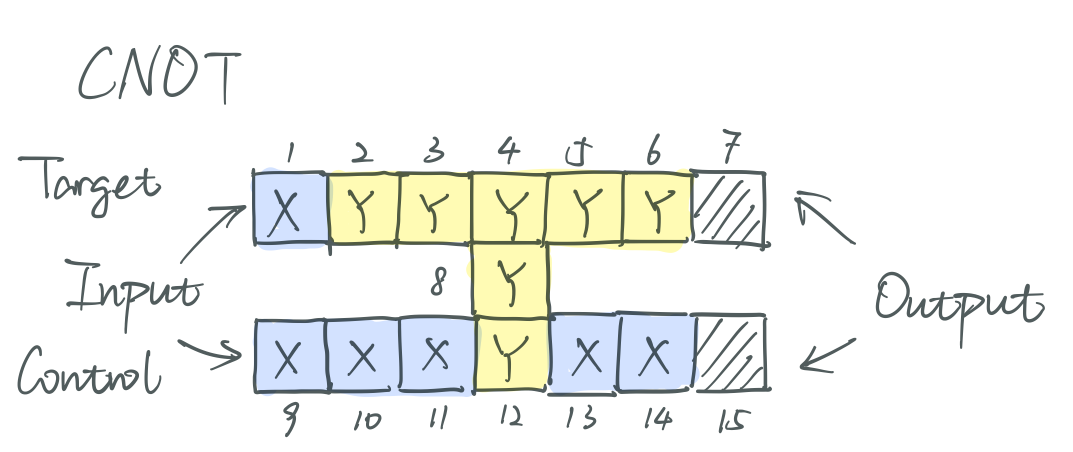
\includegraphics[width=0.5\linewidth]{CNOT.png}
\end{figure}
CNOT gate can be realized on a 15 qubit cluster state
\begin{itemize}
    \item Prepare the initial state $\ket{\psi_{in}}_{1,9}\left(\bigotimes_{i\in\mathcal{C}_{15\setminus\{1,9\}}}\ket{+}_i\right)$
    \item Entangle the 15 qubit cluster with the unitary transformation $S^{(\mathcal{C}_{15})}$
    \item One qubit measurement is performed on every qubit in the cluster except for the output qubit(7, 15).
    \begin{itemize}
        \item $\sigma_x$ measurement: qubit 1, 9, 10, 11, 13, 14
        \item $\sigma_y$ measurement: qubit 2, 3, 4, 5, 6, 8, 12
    \end{itemize}
\end{itemize}
\end{frame}

\begin{frame}{CNOT II}
\begin{figure}
    \centering
    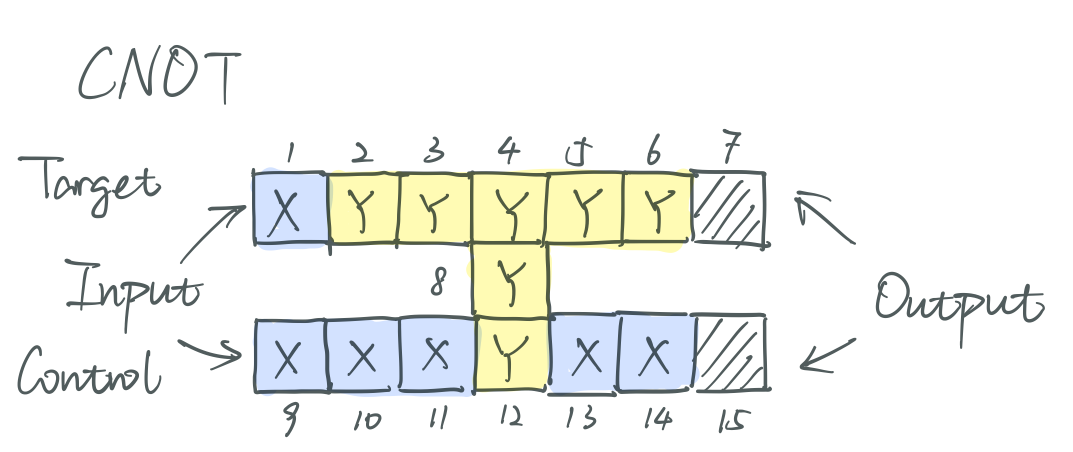
\includegraphics[width=0.5\linewidth]{CNOT.png}
\end{figure}
    \begin{itemize}
        \item The measured qubits would be destroyed and resulting gate is $U'_{CNOT} = U_{\Sigma, CNOT}CNOT(c, t)$
        \item $U_{\Sigma, CNOT} = {\sigma_x^{(c)}}^{\gamma_x^{(c)}}{\sigma_x^{(t)}}^{\gamma_x^{(t)}}{\sigma_z^{(c)}}^{\gamma_z^{(c)}}{\sigma_z^{(t)}}^{\gamma_z^{(t)}} $ with\\
        \begin{align*}
            \gamma_x^{(c)} &= s_2 + s_3 + s_5 + s_6\\
            \gamma_x^{(t)} &= s_2 + s_3 + s_8 + s_{10} + s_{12} + s_{14}\\
            \gamma_z^{(c)} &= s_1 + s_3 + s_4 + s_5 + s_8 + s_9 + s_{11} + 1\\
            \gamma_z^{(t)} &= s_9 + s_{11} + s_{13}
        \end{align*}
    \end{itemize}
\end{frame}

\begin{frame}{Construction of Quantum Gates: One-Qubit Rotation}
\begin{figure}
    \centering
    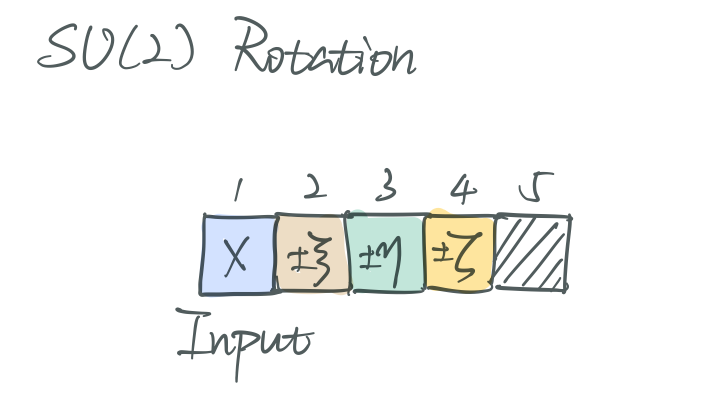
\includegraphics[width=0.5\linewidth]{Rotation.png}
\end{figure}
A general $SU(2)$ rotation $U_{Rot}[\xi, \eta, \zeta] = U_X[\zeta]U_Z[\eta]U_X[\xi]$ can be realized on 5-qubit cluster
    \begin{itemize}
        \item Prepare the state $\ket{\Psi}_{\mathcal{C}_5} = \ket{\psi_{in}}_1 \left(\bigotimes_{i = 2}^5 \ket{+}_i\right)$
        \item Create the cluster state by performing the unitary operation $S^{(\mathcal{C}_5)}$
    \end{itemize}
\end{frame}
\begin{frame}{Construction of Quantum Gates: One-Qubit Rotation}
\begin{figure}
    \centering
    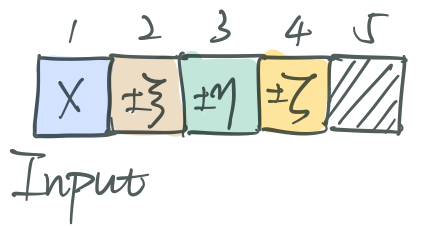
\includegraphics[width=0.5\linewidth]{Rotation2.png}
\end{figure}
    \begin{itemize}
        \item Measure the first 4 qubits in the following order. Each measurement correspond to a step of Euler rotation
            \begin{itemize}
                \item Measure qubit 1 in $\mathcal{B}_1(0)$.
                \item Measure qubit 2 in $\mathcal{B}_2(-\xi(-1)^{s_1})$.
                \item Measure qubit 3 in $\mathcal{B}_3(-\eta(-1)^{s_2})$.
                \item Measure qubit 4 in $\mathcal{B}_4(-\zeta(-1)^{s_2+s_3})$.
            \end{itemize}
        With $\mathcal{B}_j(\varphi_j) = \Bigl\{\frac{\ket{0}_i + e^{i\varphi}\ket{1}_j}{\sqrt{2}},\frac{\ket{0}_i - e^{i\varphi}\ket{1}_j}{\sqrt{2}} \Bigr\}$
        \item Then, we have performed a rotation $U'_{Rot} = U_{\Sigma,Rot}U_{Rot}[\eta, \xi, \zeta]$, with the byproduct operator $U_{\Sigma,Rot} = \sigma_x^{s_2+s_4}\sigma_z^{s_1+s_3}$
    \end{itemize}
\end{frame}

\begin{frame}{Construction of Quantum Gates: Hadamard- and $\pi/2$-Phase Gate }
\begin{figure}
    \centering
    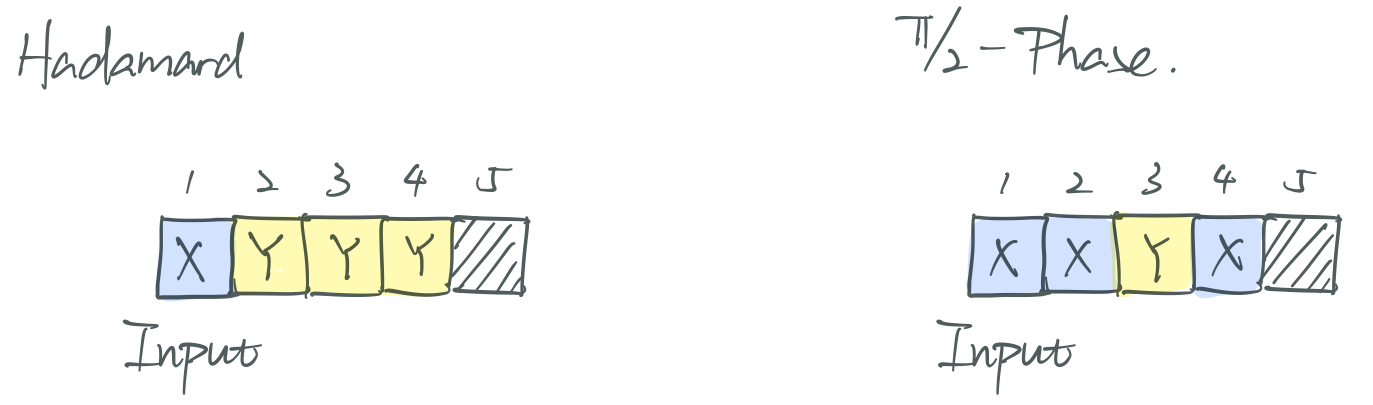
\includegraphics[width=1\linewidth]{Hadamard and Pi.png}
\end{figure}
 Hadamard and $\pi/2$-phase gate are two special cases of $SU(2)$ rotation. Hence, they can also  be realized through 5-qubit cluster.
 \begin{itemize}
     \item Prepare the 5-qubit cluster state
     \item Measurement of the first 4 qubit can be performed simultaneously
     \begin{itemize}
         \item Hadamard Gate: $\sigma_x^{(1)}$, $\sigma_y^{(2)}$, $\sigma_y^{(3)}$, $\sigma_y^{(4)}$, $U_{\Sigma, H} = \sigma_x^{s_1+s_3+s_4}\sigma_z^{s_2+s_3}$
         \item $\pi/2$-phase Gate: $\sigma_x^{(1)}$, $\sigma_x^{(2)}$, $\sigma_y^{(3)}$, $\sigma_x^{(4)}$, $U_{\Sigma, H} = \sigma_x^{s_2+s_4}\sigma_z^{s_1+s_2+s_3+1}$.
     \end{itemize}
 \end{itemize}
\end{frame}

\section{Quantum Circuit}
\begin{frame}{Quantum Circuit: Logical Network}
    How to combine quantum gates to quantum logical network?
    \begin{figure}
        \centering
        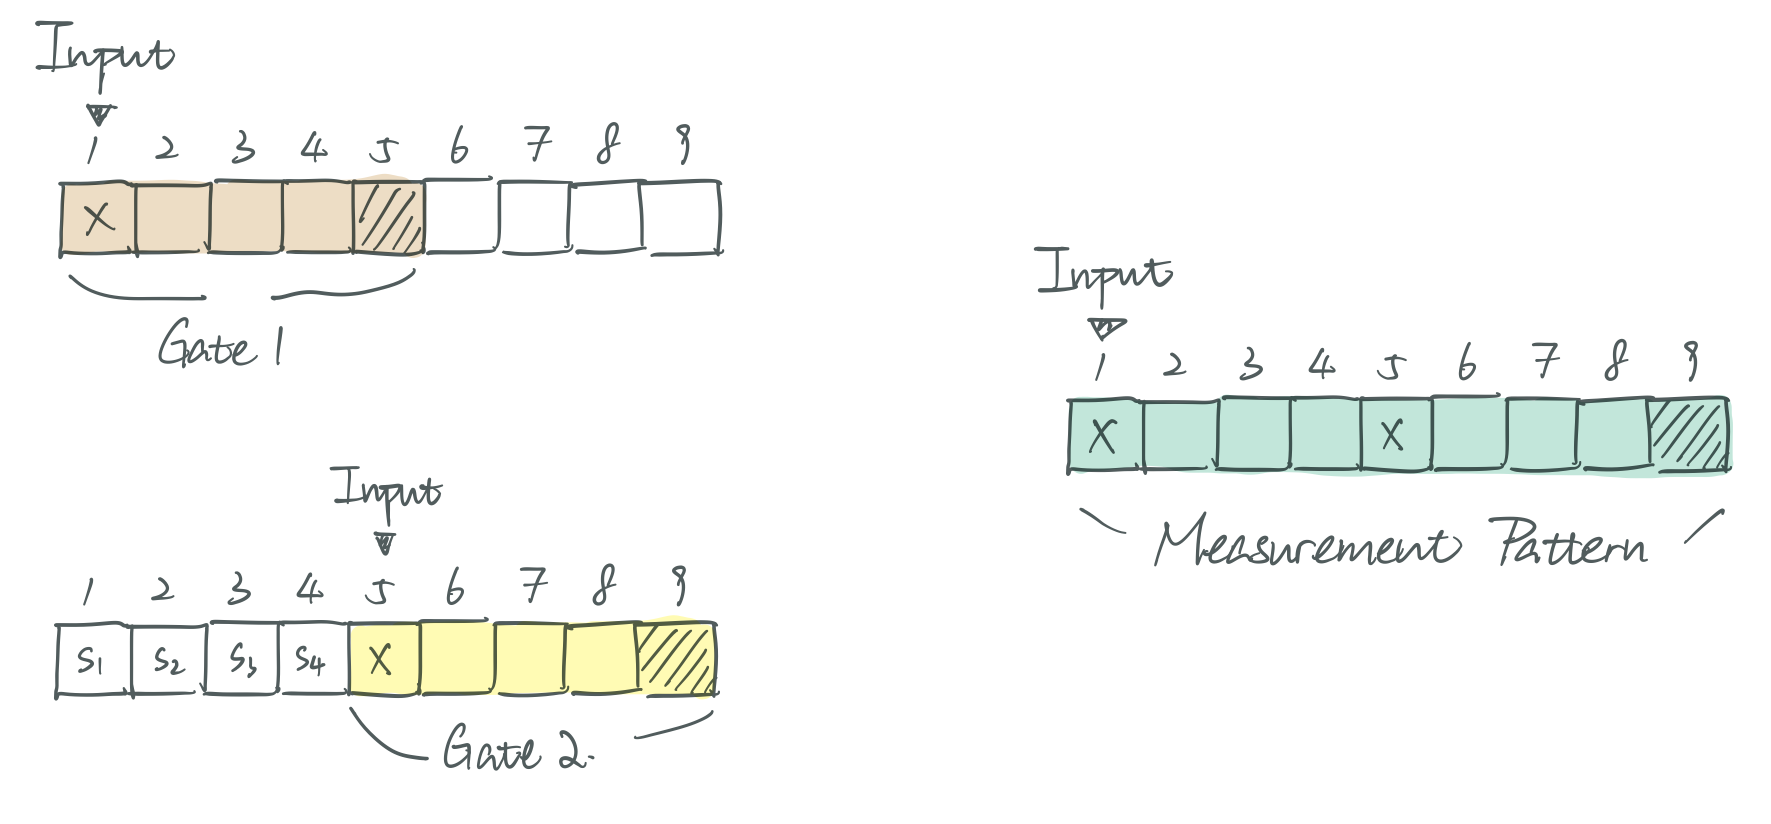
\includegraphics[width=1\linewidth]{Logical Network.png}
    \end{figure}
    \textbf{Instead of quantum gates, we have measurement patterns!}
\end{frame}

\begin{frame}[allowframebreaks]{References}
      \bibliography{bib}
  \bibliographystyle{apalike}

  \nocite{*}
\end{frame}

\end{document}
